
\chapter{Basic concepts in estimation}
\label{chap:theory}

An estimation problem in statistics may have many potential solutions. To
separate useful estimation strategies from approaches that are less feasible,
criteria have to be defined by which different estimators can be evaluated and
compared. In this chapter we first review a number of basic criteria typically
used in classic statistics. We then discuss additional criteria that are
important in the context of robust statistics. Our discussion in this chapter
is conceptual in nature; it is supposed to establish a theoretical basis for
the specific robust estimators that are discussed in the subsequent chapters
from an applied perspective.

\section{Classical properties of estimators}

The goal of statistical estimation is to obtain a reasonable value for the
unknown \emph{paramater} of a statistical model, based data whose properties
are assumed to be consistent with the suggested model. Let $\mathcal{X}^{(n)} =
\{\stvec{x}_1, \dots, \stvec{x}_n\}$                                            \todo{Do we need the parentheses around $n$? 
                                                                                (In general, to improve readability, we should use
                                                                                as little ink as possible in equations.) Later 
                                                                                in the chapter, $n$ is a subscript (without 
                                                                                parentheses) not a superscript; what would be the 
                                                                                best way to deal with $n$?}
be a set of $n$ random variables $\stvec{x}_1, \ldots, \stvec{x}_n$ that have a joint
probability distribution $P_{\boldsymbol\theta}^{(n)}$ depending on the unknown
parameter $\boldsymbol\theta$. Note that, depending on context,
$\boldsymbol\theta$ may be scalar, or it may be a vector of multiple parameters,
that is $\boldsymbol\theta = (\theta_1, \dots, \theta_p)'$. Likewise, $\stvec{x}_i$
may be univariate, or it may contain multiple dimensions, that is $\stvec{x}_i =
(X_{i1}, \dots, X_{ik})'$. \alert{[I think it is important to
emphasize that $X$ can be a collection of variables as the book is on
regression and not on univariate statistics. Hence, I changed notation to vectors.
But I'm unsure whether this is ok...]}

We assume that the joint distribution of the random variables $\stvec{x}_i$, $i=1,
\dots, n$, belongs to the (parametric) statistical model $\mathcal{P}^{(n)} =
\{P_{\boldsymbol\theta}^{(n)} | \boldsymbol\theta \in \boldsymbol\Theta\}$,     \todo{I do not really understand. Why do we need 
                                                                                $\mathcal{P}$? What is the difference to 
                                                                                $P_{\boldsymbol\theta}$?}
where $\boldsymbol\Theta$ is the set of possible values of $\boldsymbol\theta$. \todo{Maybe be a bit more specific about 
                                                                                $\boldsymbol\Theta$. I made Theta bold because if 
                                                                                $\boldsymbol\theta$ is multidimensional then also 
                                                                                $\boldsymbol\Theta$ has to be. Or do I misunderstand 
                                                                                what Theta is?}
The goal is to estimate $\boldsymbol\theta \in \boldsymbol\Theta$ based on a
realization of $\mathcal{X}^{(n)}$. In general, we will consider the case in
which the statistical model $\mathcal{P}^{(n)}$ conforms to simple random
sampling (\stsc{SRS}), that is, a situation in which the random variables
$\stvec{x}_1, \dots, \stvec{x}_n$ are independent and identically distributed
(i.i.d.). In this situation, each $\stvec{x}_i$ independently follows a common
distribution $P_{\boldsymbol\theta}$, which can be characterized by the
distribution function $F_{\boldsymbol\theta}(\stvec{x}) = \Pr(X_1 \leq x_1,
\dots, X_k \leq x_k)$ (or simply $F$ when there is no risk of confusion about
the parameter we have to estimate).

An \emph{\Index{estimator}} of $\boldsymbol\theta$ can then be defined as
follows: An \Index{estimator} of the parameter $\boldsymbol\theta$ is any
statistic $\sthat{\boldsymbol\theta} =
\sthat{\boldsymbol\theta}(\mathcal{X}^{(n)})$ taking its value in
$\boldsymbol\Theta$.

The value of $\sthat{\boldsymbol\theta}$ provided by a particular realization
of the random variables $\stvec{x}_1, \dots, \stvec{x}_n$ is called an
\emph{\Index{estimate}} of $\boldsymbol\theta$. Note that, for simplicity, we
will often use the notation $\stvec{x}_i$, $i = 1, \dots, n$, to designate the
$i$th random variable as well as a realization of it (i.e., a specific
observation); the context will always clearly indicate if we have to consider
$\stvec{x}_i$ as a random variable or as a particular value.

The definition above contains no indication of the quality of an estimator; any
statistic $\sthat{\boldsymbol\theta}$ that provides a value in
$\boldsymbol\Theta$ is a valid estimator. To narrow down the set of estimators
to estimators that can be considered useful we need quality criteria. Classic
quality criteria are unbiasedness, efficiency, and consistency.

\subsection{Unbiasedness}
\Index[unbiasedness]{}

From a good estimator one may expect that, on average, it gives the “correct”
answer. Let us denote by
$E_{\boldsymbol\theta}(\sthat{\boldsymbol\theta}(\mathcal{X}^{(n)}))$ the
expectation of statistic $\sthat{\boldsymbol\theta}(\mathcal{X}^{(n)})$ when
$\mathcal{X}^{(n)} \sim P_{\boldsymbol\theta}^{(n)}$. Think of
$E_{\boldsymbol\theta}$ as the average value we would obtain for
$\sthat{\boldsymbol\theta}$ from a large number of repeated realizations of
$\mathcal{X}^{(n)}$, given that for each repetition $\mathcal{X}^{(n)}$ follows
distribution $P_{\boldsymbol\theta}^{(n)}$ (as, for example, in repeated random
sampling from the same population).

Unbiasedness can then be defined as follows:
The estimator $\sthat{\boldsymbol\theta} = \sthat{\boldsymbol\theta} 
(\mathcal{X}^{(n)})$ is called unbiased if
\[
    E_{\boldsymbol\theta}(\sthat{\boldsymbol\theta}) = \boldsymbol\theta
    \qquad
    \text{for all $\boldsymbol\theta \in \boldsymbol\Theta$ and all $n$}
\]

That is, no matter the sample size $n$, estimator $\sthat{\boldsymbol\theta}$
will, on average across a large number of repeated samples, provide the correct
answer (given that our assumptions about the joint distribution of
$\mathcal{X}^{(n)}$ are correct, such as, e.g., independent sampling of
observations). The difference
\[
    B_{\boldsymbol\theta}(\sthat{\boldsymbol\theta}) 
        = E_{\boldsymbol\theta}(\sthat{\boldsymbol\theta}) - \boldsymbol\theta
\]
is called the \emph{\Index{bias}} of estimator $\sthat{\boldsymbol\theta}$.
The absence of bias indicates that the sampling distribution of
$\sthat{\boldsymbol\theta}$ has a mean that coincides with the value of the
parameter of interest.

Zero bias is often difficult to achieve in small samples. Therefore, another
useful criterion is \emph{asymptotic unbiasedness}: The estimator
$\sthat{\boldsymbol\theta} = \sthat{\boldsymbol\theta}(\mathcal{X}^{(n)})$ is
called asymptotically unbiased if
\[
    \lim_{n \rightarrow \infty} E_{\boldsymbol\theta}(\sthat{\boldsymbol\theta}) = \boldsymbol\theta
    \qquad
    \text{for all $\boldsymbol\theta \in \boldsymbol\Theta$}
\]

That is, an estimator is asymptotically unbiased if the bias vanishes with 
increasing sample size. An important question in this context is, of course, how 
fast the bias vanishes (or how large the sample size has to be for the bias to be 
negligible).

\subsection{Efficiency}

For a specific estimation problem, several (asymptotically) unbiased estimators
may exist. To choose the best among them we need further information about the
performance of the different estimators. Furthermore, there may also be
situations in which a biased estimator is to be preferred over an unbiased
estimator. A key aspect in this regard is the \emph{\Index{efficiency}} of an
estimator. Efficiency has to do with how spread out about $\boldsymbol\theta$
the sampling distribution of the estimator is. The smaller the dispersion of
estimator $\sthat{\boldsymbol\theta}$ around the true value
$\boldsymbol\theta$ in repeated samples, the more “efficient” (or precise) is
the estimator.

\paragraph{Mean squared error}

First consider the case of a \emph{scalar} parameter $\theta$. The
precision of estimator $\sthat{\theta}$ can be measured by its
\emph{\Index{mean squared error}} (\stsc{MSE}):
\[
    \stsc{MSE}_{\theta}(\sthat{\theta}) 
    = E_{\theta} \left((\sthat{\theta} - \theta)^2\right)
\]
A small mean squared error for $\sthat{\theta}$ means that the sampling
distribution of $\sthat{\theta}$ is well concentrated around the exact value
of the parameter to estimate and hence that the estimator $\sthat{\theta}$
has a good precision.

It is easy to show that
\[
    \stsc{MSE}_{\theta}(\sthat{\theta})
    = \mathrm{Var}_{\theta}(\sthat{\theta}) 
      + \left(B_{\theta}(\sthat{\theta})\right)^2
\]
That is, the mean squared error of an estimator can be decomposed into its
variance and its squared bias. Hence, if $\sthat{\theta}$ is unbiased,
$\stsc{MSE}_{\theta}(\sthat{\theta})$ is simply equal to
$\mathrm{Var}_{\theta}(\sthat{\theta})$.

\paragraph{Relative efficiency}

An estimator $\sthat{\theta}_A$ of $\theta$ is more precise---we will say
\emph{more efficient}---than another estimator $\sthat{\theta}_B$ if
\[
    \stsc{MSE}_{\theta}(\sthat{\theta}_A) \leq 
    \stsc{MSE}_{\theta}(\sthat{\theta}_B)
    \qquad\text{for all $\theta \in \Theta$}
\]
\alert{and                                                                     \todo{Shouldn't it be “$<$” in at least one case?}
\[
    \stsc{MSE}_{\theta}(\sthat{\theta}_A) < 
    \stsc{MSE}_{\theta}(\sthat{\theta}_B)
    \qquad\text{for at least one $\theta \in \Theta$}
\]
}

In general, we consider the “large-sample” sampling distributions of
asymptotically unbiased estimators. If, for large $n$, the estimators
$\sthat{\theta}_A$ and $\sthat{\theta}_B$ are approximately
$\mathcal{N}(\theta, \textrm{Var}(\sthat{\theta}_A))$ and
$\mathcal{N}(\theta, \textrm{Var}(\sthat{\theta}_B))$, respectively, we
define the \emph{\Index{asymptotic relative efficiency}} (\stsc{ARE}) of
$\sthat{\theta}_B$ with respect to $\sthat{\theta}_A$ as the ratio
\[
    \stsc{ARE}_{\theta}(\sthat{\theta}_B,\sthat{\theta}_A) 
    = \frac{ \textrm{Var}(\sthat{\theta}_A)}{\textrm{Var}(\sthat{\theta}_B)}
\]
(see \citealp{Serfling1980}). If $\sthat{\theta}_B$ is (asymptotically) less
efficient than $\sthat{\theta}_A$, then
\[
    \stsc{ARE}_{\theta}(\sthat{\theta}_B,\sthat{\theta}_A) < 1
\]


\paragraph{Efficiency of the maximum likelihood estimator}

Let us consider the case in which the random variables
$\stvec{x}_1, \ldots, \stvec{x}_n$ are univariate and i.i.d.\ with a common
distribution function $F_{\theta}$ and a common density function $f_{\theta}$
that satisfies some differentiability conditions with respect to $\theta$.
Suppose also that the \emph{\Index{Fisher information}}
\[
    \mathcal{I}\left(F_{\theta}\right) =
        E_{\theta}\left(\left(\frac{\partial}{\partial\theta}
        \log f_{\theta}(\stvec{x})\right)^2\right)
\] 
is strictly positive and finite. Then it follows that
\begin{enumerate}
    \item[(i)] for large $n$, the maximum likelihood estimator
    $\sthat{\theta}_{\stsc{ML}}$ of $\theta$ is approximately distributed as
    $\mathcal{N}\left(\theta, (n \mathcal{I}(F_{\theta}))^{-1}\right)$
    
    \item[(ii)] for a wide class of estimators $\sthat{\theta}$ that are
    approximately distributed as $\mathcal{N}(\theta, V)$, a \emph{lower
    bound} to $V$ is $(n \mathcal{I}(F_{\theta}))^{-1}$
\end{enumerate}
(see \citealp{LehmannCasella1988}). In this situation,
%
\begin{equation}\label{eq:ARE_vsML}
    \stsc{ARE}_{\theta}(\sthat{\theta}, \sthat{\theta}_{\stsc{ML}})
     = \frac{(n \mathcal{I}(F_{\theta}))^{-1}}{V} \leq 1
\end{equation}
%
making $\sthat{\theta}_{\stsc{ML}}$ the most (asymptotically) efficient among
the given class of estimators $\sthat{\theta}$. Note, however, as will be
discussed later, that (\ref{eq:ARE_vsML}) does not necessarily make
$\sthat{\theta}_{\stsc{ML}}$ the estimator of choice, when certain other
considerations are taken into account.


\paragraph{Notation in the multidimensional case}

If $\boldsymbol\theta = (\theta_1, \dots, \theta_p)'$ is a vector of parameters
we define the \emph{\Index[mean squared error!matrix]{mean squared error matrix}}
of the estimator $\sthat{\boldsymbol\theta}$ as follows:
\[
    \stsc{MSE}_{\boldsymbol\theta}(\sthat{\boldsymbol\theta})
    = E_{\boldsymbol\theta}\left((\sthat{\boldsymbol\theta} - \boldsymbol\theta)
                                 (\sthat{\boldsymbol\theta} - \boldsymbol\theta)'
                           \right)
\]
If $\sthat{\boldsymbol\theta}$ is unbiased, the mean squared error matrix simply
coincides with the covariance matrix of the estimator.

If, for large $n$, the $p$-variate estimators $\sthat{\boldsymbol\theta}_A$ and
$\sthat{\boldsymbol\theta}_B$ are approximately normally distributed with mean
$\boldsymbol\theta$ and nonsingular covariance matrices $\boldsymbol\Sigma_A$ and
$\boldsymbol\Sigma_B$, respectively, it is usual to define the 
\emph{\Index{asymptotic relative efficiency}} (\stsc{ARE}) of
$\sthat{\boldsymbol\theta}_B$ with respect to $\sthat{\boldsymbol\theta}_A$ as
the ratio of the \emph{generalized variances} (determinants of the covariance
matrices), raised to the power $1/p$, that is
\[
    \stsc{ARE}_{\boldsymbol\theta}(\sthat{\boldsymbol\theta}_B, \sthat{\boldsymbol\theta}_A)
    = \left(\frac{ \det(\boldsymbol\Sigma_A)}{\det(\boldsymbol\Sigma_B)}\right)^{1/p}
\]
If $\stsc{ARE}_{\boldsymbol\theta}(\sthat{\boldsymbol\theta}_B,
\sthat{\boldsymbol\theta}_A)<1$, estimator $\sthat{\boldsymbol\theta}_B$ is
(asymptotically) less efficient than estimator $\sthat{\boldsymbol\theta}_A$.

Here again the maximum likelihood estimator $\sthat{\boldsymbol\theta}_\stsc{ML}$ of
$\boldsymbol\theta$ appears as the most (asymptotically) efficient estimator among a
wide class of (asymptotically) unbiased estimators $\sthat{\boldsymbol\theta}$ of
$\boldsymbol\theta$. Moreover, for large $n$,
\[
    \sthat{\boldsymbol\theta}_\stsc{ML} \approx 
    \mathcal{N}\left(\boldsymbol\theta, (n \stmat{I}(F_{\boldsymbol\theta}))^{-1}\right)
\]
where “$\approx$” stands for “is approximately distributed as” and
$\stmat{I}(F_{\boldsymbol\theta})$ is the $p\times p$ Fisher information matrix
with its elements defined as
\[
    \mathcal{I}_{ij}\left(F_{\boldsymbol\theta}\right) =
    E_{\boldsymbol\theta}\left(
    \frac{\partial}{\partial\theta_i}\log f_{\boldsymbol\theta}(\stvec{x}) \cdot 
    \frac{\partial}{\partial \theta_j}\log f_{\boldsymbol\theta}(\stvec{x})
    \right)
\] 


\subsection{Consistency}
\Index[consistency]{}

The consistency criterion comes in two flavors, as consistency in terms of
convergence in probability and as consistency in terms of convergence in
distribution. \alert{[Please explain here (or below) why (asymptotic)
unbiasedness and efficiency is not enough an why the additional criterion of
consistency is needed.]}

\paragraph{Convergence in probability}
\Index[convergence!in probability]{}

An estimator $\sthat{\boldsymbol\theta} =
\sthat{\boldsymbol\theta}(\mathcal{X}^{(n)})$ is \emph{consistent} if, for $n
\rightarrow \infty$, $\sthat{\boldsymbol\theta}$ \emph{converges in
probability} to $\boldsymbol\theta$. That is, for any $\epsilon > 0$ and for
all $\boldsymbol\theta \in \boldsymbol\Theta$:
\[
    \lim_{n \rightarrow \infty} P_{\boldsymbol\theta}^{(n)} \left(
        \Vert\sthat{\boldsymbol\theta} - \boldsymbol\theta \Vert \leq \epsilon
        \right) = 1
\]

This type of consistency means that, when the sample size grows, the
probability that the estimator $\sthat{\boldsymbol\theta}$ takes a value near
the exact value of the parameter and, consequently, provides a “good” estimate
of the parameter $\boldsymbol\theta$, grows to 1. Consistency of                \todo{I don't really understand this sentence (“Consistency of \dots”)}
$\sthat{\boldsymbol\theta}$ is required if we want an estimator to provide
unambiguous statistical inference for $\boldsymbol\theta$.
Note that consistency in terms convergence in probability is given if an
estimator is asymptotically unbiased and if the
variance of the estimator approaches zero as the sample size grows.

For simplicity, consider the case of a scalar parameter $\theta$. If            \todo{I don't understand. What is “convergence in quadratic mean”? Where does $L_2$ come from?}
$B_{\theta}(\sthat{\theta}) \stackrel{n \rightarrow \infty}{\longrightarrow} 0$
and $\mathrm{Var}_{\theta}(\sthat{\theta}) \stackrel{n \rightarrow
\infty}{\longrightarrow} 0$, then $\stsc{MSE}_{\theta}(\sthat{\theta})
\stackrel{n \rightarrow \infty}{\longrightarrow} 0$, so that $\sthat{\theta} =
\sthat{\theta}(\mathcal{X}^{(n)})$ \emph{\Index[convergence!in
quadratic mean]{converges in quadratic mean}} to $\theta$. That is, for $n
\rightarrow \infty$, $\sthat{\theta} \stackrel{L_2}{\rightarrow} \theta$. It is
well known that convergence in quadratic mean implies convergence in
probability.

\paragraph{Convergence in distribution}
\Index[convergence!in distribution]{}

The statistic $T^{(n)} = T(\mathcal{X}^{(n)})$ \emph{converges in distribution}
to the probability distribution $\mathcal{L}$ if, for $n \rightarrow \infty$,
the distribution function $F_{T^{(n)}}$ of $T^{(n)}$ converges to the
distribution function $F_\mathcal{L}$ of $\mathcal{L}$ in any point of
continuity of $F_\mathcal{L}$. That is, convergence in probability is
given if
\[
    F_{T^{(n)}}(x) \stackrel{n \rightarrow \infty}{\longrightarrow} F_\mathcal{L}(x)
    \quad\text{for any continuity point $x$ of distribution function $F_\mathcal{L}$}
\]

As a shorthand, we will write
\[
    T^{(n)} \stackrel{d}{\rightarrow} \mathcal{L}
\]
to denote convergence in probability for $n \rightarrow \infty$. In practice, 
convergence in probability means that, for large $n$, we may consider that
$T^{(n)}$ is approximately distributed as $\mathcal{L}$, that is,
\[
    T^{(n)} \approx \mathcal{L}
\]

\alert{[Please explain here why convergence in probability is a useful
concept. What is it used for? Why do we need it in the context of robust
statistics?]}

\alert{[What about Fisher-consistency?]}

\subsection{Other aspects}

Depending on context, a number of other criteria can be important. For example,
from a practical perspective, \emph{computational complexity} can be a relevant
criterion to choose between different estimators. In general, estimators that
require operations in the order of $n^2$ (that is, if the number of required
computational operations grows quadratically with the sample size) lead to
prohibitive computational costs in large samples. In many cases it is possible
to design alternative estimators (or improved computational algorithms
for a given estimator) that only require operations in the order of $\ln n$ and
are thus much more efficient (with respect to computer time) in large samples.
\alert{[Maybe expand a bit on this.]}

Furthermore, consistent estimators may differ in their \emph{rate of
convergence}, that is, in how fast the mean squared error diminishes with
growing sample size. \alert{[Please expand on this. How is the rate of
convergence defined (and interpreted)? What are typical rates of convergence,
e.g. of the mean etc.?]} Naturally, an estimator with a faster rate of
convergence, is usually to be preferred over an estimator with a slower rate of
convergence. \alert{[Does this make sense?]}

To enable approximately valid statistical inference in terms of confidence
intervals and significance tests, a further important criterion is
\emph{asymptotic normality}. Asymptotic normality is given if it can be shown
that the sampling distribution of an estimator approximates the normal
distribution in large samples. For example, maximum-likelihood estimators can
be shown to be asymptotically normal under general conditions. If,
however, the asymptotic sampling distribution of an estimator is known to be 
non-normal, the viability of the estimator for statistical inference is 
limited.\alert{[Does this make sense? Please expand ...]}

Finally, an estimator should be \emph{equivariant} to transformations of data.
That is, a transformation of the data should affect the estimator
$\sthat{\boldsymbol\theta}$ in the same functional way as it affects the true
parameter $\boldsymbol\theta$. For example, let $\theta_A$ be the expected
value of variable $X_A$ and $\theta_B$ be the expected value of variable $X_B$.
If $X_B$ can be expressed as a linear combination of $X_A$, that is, $X_B = a +
b \cdot X_A$, then $\theta_B = a + b \cdot \theta_A$. In this case, also
$\sthat{\theta_B} = a + b \cdot \sthat{\theta_A}$ should hold. In other words,
whether you express your data in Dollars or in Euros, whether you express your
data in degrees Fahrenheit or degrees Celsius should only affect the scaling of
your estimator, but should not affect your results otherwise.

\alert{[I just wrote some stuff in this section about points that seem 
relevant to me. I am not sure whether I always chose the right words. Also, maybe 
it would be good express some of it formally.]}


\section{Measures of robustness}

Intuitively, the classical approach to statistics is about defining estimators
that have desirable properties under clearly specified conditions. The goal of
robust methods, however, is to develop estimators that perform well also in the
“neighborhood” of such conditions. This leads to the proposition of so called
“robust” estimators, that are, for instance, not affected too strongly or too
quickly by the presence of outliers. Although outliers are only one of
the main concerns of robust methods, we will make our first steps into
robustness theory by presenting some basic concepts for measuring the degree to
which estimators are affected by atypical observations.


\begin{stexample}
    Consider the following observations of the grades achieved by $n = 25$ students
    in fifth year of primary school (on a scale of 1 to 10):                        \todo{Is 1-10 correct?}
    
    \begin{center}
    \begin{tabular}{rrrrrr}%
    6.00 & 6.50 & 7.00 & 7.00 & 7.00\\
    7.00 & 7.00 & 7.50 & 7.50 & 8.00\\
    8.00 & 8.00 & 8.50 & 8.50 & 8.50\\
    8.50 & 9.00 & 9.00 & 9.50 & 9.50\\
    9.50 & 9.50 & 9.50 & 9.50 & 10.00
    \end{tabular}
    \end{center}
    
    If we calculate two \emph{measures of location}, the \Index{mean} and the
    \Index{median}, as well as two \emph{measures of scale}, the
    \Index{standard deviation} and the \Index{interquartile range}, the results
    are as follows:
    
\begin{stlog}
. drop _all
{\smallskip}
. matrix x = (6.00, 6.50, 7.00, 7.00, 7.00,    ///
>             7.00, 7.00, 7.50, 7.50, 8.00,    ///
>             8.00, 8.00, 8.50, 8.50, 8.50,    ///
>             8.50, 9.00, 9.00, 9.50, 9.50,    ///
>             9.50, 9.50, 9.50, 9.50, 10.00)'
{\smallskip}
. quietly svmat x
{\smallskip}
. tabstat x, statistics(mean median sd iqr)
{\smallskip}
    variable {\VBAR}      mean       p50        sd       iqr
\HLI{13}{\PLUS}\HLI{40}
          x1 {\VBAR}      8.22       8.5  1.137248       2.5
\HLI{13}{\BOTT}\HLI{40}
{\smallskip}

\end{stlog}
    
    Now, imagine the dot separating the decimals in the last observation is
    mistakenly removed, so that the last observation is coded as 1000. In this 
    case the results are the following:
    
\begin{stlog}
. use Star.dta, clear
{\smallskip}
. regress log_intensity log_temperature
{\smallskip}
      Source {\VBAR}       SS           df       MS      Number of obs   =        47
\HLI{13}{\PLUS}\HLI{34}   F(1, 45)        =      2.08
       Model {\VBAR}  .664593334         1  .664593334   Prob > F        =    0.1557
    Residual {\VBAR}  14.3463934        45  .318808743   R-squared       =    0.0443
\HLI{13}{\PLUS}\HLI{34}   Adj R-squared   =    0.0230
       Total {\VBAR}  15.0109868        46  .326325799   Root MSE        =    .56463
{\smallskip}
\HLI{14}{\TOPT}\HLI{64}
log_intensity {\VBAR}      Coef.   Std. Err.      t    P>|t|     [95\% Conf. Interval]
\HLI{14}{\PLUS}\HLI{64}
log_tempera{\tytilde}e {\VBAR}  -.4133041   .2862575    -1.44   0.156    -.9898562     .163248
        _cons {\VBAR}   6.793468   1.236516     5.49   0.000     4.302998    9.283939
\HLI{14}{\BOTT}\HLI{64}
{\smallskip}

\end{stlog}
    
    As is evident, the \Index{mean} and the \Index{standard deviation} strongly
    increased due to the introduction of the erroneous observation, whereas
    the \Index{median} and the \Index{interquartile range} remained unchanged.
    The example illustrates the fact that one single outlier may “break” the
    \Index{mean} and the \Index{standard deviation}, but does not affect the
    \Index{median} or the \Index{interquartile range}. Hence, these two later
    statistics can be considered as being more robust to erroneous data than
    the two first ones.

    % Let $x_i$, $j=1, \dots, n$, denote the (unordered) data. Furthermore, let
    % $x_{(i)}$ be the $i$th observation in the list of ordered data (i.e.\
    % $x_{(1)}\leq\dots\leq x_{(n)}$) and let $\lceil x \rceil$ denote the
    % smallest integer greater or equal to $x$. We can then calculate two
    % \emph{measures of location}, the \Index{mean} $\mu$ and the
    % \Index{median} $Q_{0.5}$, as follows:
    % \[
    %     \mu = \frac{1}{n}\sum_{i=1}^n x_i = 8.22
    %     \qquad\qquad
    %     Q_{0.5} = x_{(\lceil 25/2 \rceil)} = x_{(13)} = 8.50
    % \]
    %
    % Furthermore, two \emph{measures of scale}, the \Index{standard deviation}
    % $\sigma$ and the \Index{interquartile range} $\stsc{IQR}$, are given
    % as:
    % \begin{align*}
    %     \sigma       &= \sqrt{\frac{1}{n} \sum_{i=1}^n (x_i - \mu)^2} = 1.11\\[1ex]
    %     \stsc{IQR}   &= Q_{0.75} - Q_{0.25}
    %                     = x_{(\lceil 25 \cdot 0.75\rceil)}-x_{(\lceil 25 \cdot 0.25\rceil)}
    %                     = x_{(19)} - x_{(7)}\\
    %                    &= 9.50 - 7.00 = 2.50
    % \end{align*}
    %
    % Now, imagine the dot separating the decimals in the last observation is
    % mistakenly removed, so that the last observation is coded as 1000. In this
    % case, the \Index{mean} increases to 47.82, but the \Index{median} is not
    % affected by the erroneous data and remains at 8.50. Furthermore, the
    % \Index{standard deviation} moves from 1.11 to 194.37, while the
    % \Index{interquartile range} remains unchanged. This example illustrates the
    % fact that one single outlier may “break” the sample \Index{mean}
    % and the \Index{standard deviation}, but does not affect the sample
    % \Index{median} or the \Index{interquartile range}. Hence, these two later
    % statistics can be considered as being more robust to erroneous data than
    % the two first ones.
\end{stexample}

How can the degree of robustness of different statistics be quantified? How can
we compare the robustness of different estimators from various viewpoints?
These are questions we will address in the rest of this section.

In robust estimation theory it is common to consider \emph{parameters} as
\emph{functionals}. More precisely, the functional by which a parameter $T$ is
defined is a rule that maps every probability distribution $F$ into a real
number, that is $T = T(F)$.\footnote{$F$ is the cumulative distribution
function of a random variable $X$. Evaluated at position $x$, the function
returns the probability that the random variable will take on a value lower
than or equal to $x$, that is, $F(x) = \Pr(X \leq x)$. In order to avoid
unnecessary technical difficulties we will generally assume in this chapter
that the distribution $F$ is continuous with density $f$. The density is the
first derivative of $F$; it is nonnegative and integrates to one.} Often, a
natural \emph{estimate} $T_n$ of the parameter $T(F)$ based on sample
$\mathbf{X}_n= \{x_1, \dots, x_n\}$---where $x_1, \dots, x_n$ are realizations
of $n$ independent and identically distributed (i.i.d.) random variables $X_1,
\dots, X_n$ of distribution $F$---may be defined as the value of the functional
at the empirical distribution $F_n$.\footnote{The empirical distribution $F_n$
is a discrete distribution with a probability mass of $1/n$ at each value of
the sample $\mathbf{X}_n$.} That is,
$T_n = T(F_n)$. For example, if
\[
    T(F) = \int_{-\infty}^\infty x \dif F(x) = \mu
\]
\[
    T(F) = \int_{-\infty}^\infty x \dif F(x) = \mu
\]
is the expected value of the distribution $F$, then
\[
    T_n = T(F_n) = \int_{-\infty}^\infty x \dif F_n(x) 
          = \frac{1}{n} \sum_{i=1}^n x_i = \mu_n
\]
is the arithmetic \Index{mean} of a sample $\mathbf{X}_n$ from $F$. Likewise, if $T(F) =
F^{-1}(0.5) = Q_{0.5}$ is the \Index{median} of the distribution $F$, then $T_n =
T(F_n) = F_n^{-1}(0.5) = Q_{0.5;n}$ is the empirical median of a sample
$\mathbf{X}_n$ from $F$.

The robustness of a statistic (or estimator) $T_n$ may be analyzed in a very
intuitive way by studying how a contamination of the sample
$\mathbf{X}_n$ affects $T_n$. This empirical approach leads to the notions of
the \emph{\Index{sensitivity curve}} and the \emph{\Index[breakdown
point!finite-sample]{finite-sample breakdown point}} of $T_n$. But it is also
of great interest to consider the limiting case where $n$ tends to infinity. As
the sample size $n$ grows, the empirical distribution function $F_n$ approaches
the underlying population distribution function $F$, and the empirical measures
of robustness of the statistic $T_n$ move in a natural way to the concepts of
the \emph{\Index{influence function}} and the \emph{\Index[breakdown
point!asymptotic]{asymptotic breakdown point}} of the functional $T$.


\subsection{The sensitivity curve and the influence function}
\label{subsec:theory:IF}

\subsubsection{The sensitivity curve}
\index{subject}{sensitivity curve|(textbf}

The \textit{sensitivity curve} (\stsc{SC}) is an empirical tool to quantify the
robustness of a statistic in a given sample. Consider a data set
$\mathbf{X}_n = \{x_1, \dots, x_n\}$ and the statistic $T_n =
T_n(x_1, \dots, x_n) = T(F_n)$. To study the impact of a potential
outlier on this statistic, we may analyze the change in the value of the
statistic once we add an extra data point $x$, where $x$ is varied between
$-\infty$ an $+\infty$. Hence, the \emph{(standardized) sensitivity curve} of
statistic $T_n$ for the sample $\mathbf{X}_n$ is defined as
\[
    \stsc{SC}(x; T_n, \mathbf{X}_n) = 
    \frac{T_{n+1}(x_1, \dots, x_n, x) - T_n(x_1, \dots, x_n)}{\frac{1}{n+1}}
\]
That is, for each value of $x$ we compare the statistic in the “contaminated”
sample to its value in the original sample, and rescale the difference by
dividing the difference by $1/(n+1)$, the proportion of contamination.

\begin{stexample}
Consider a data set $\mathbf{X}_n$ of $n=20$ (rounded) random numbers from a
$\mathcal{N}(0,1)$ (standard normal) distribution:
\begin{center}\begin{tabular}{*{10}{D{.}{.}{2.2}}}
    -0.49 &      0.14 &      1.54 &      0.63 &     -0.87 &     -0.86 &      1.65 &     -0.55 &      0.91 &     -0.03 \\
    -0.61 &      0.22 &     -1.61 &      0.15 &      0.36 &      1.96 &      1.04 &      0.24 &     -0.45 &      0.98
\end{tabular}\end{center}

Figure \ref{fig:theory:SClocation} shows the standardized sensitivity curves
for the \Index{mean} and the \Index{median}; Figure \ref{fig:theory:SCscale}
displays the standardized sensitivity curves for the \Index{standard deviation}
and the \Index{interquartile range}. As is evident, the \Index{mean} and the
\Index{standard deviation} have unbounded sensitivity curves (the curves go off
to minus or plus infinity as the outlier moves away from the center of
the uncontaminated data), whereas the sensitivity curves of the \Index{median}
and the \Index{interquartile range} are bounded. The “classic” location and
scale measures may be completely perturbed by the presence of one single
outlying observation---this illustrates the non-robust character of these two
statistics---, while the impact of the additional outlying observation on the
quantile-based location and scale measures remains very limited.
\end{stexample}


\begin{figure}[h!]
    \centering
    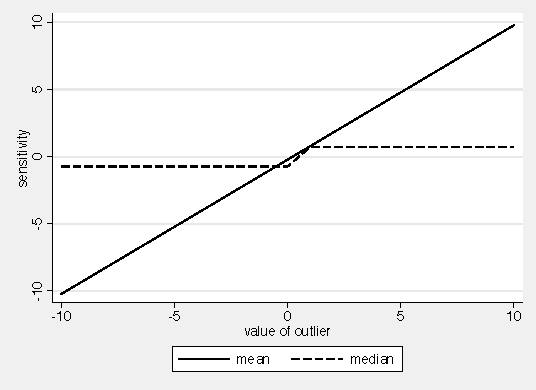
\epsfig{file=eps/2/4}
    \caption{Standardized sensitivity curves of the mean and the median for a sample of $n=20$ random $\mathcal{N}(0,1)$ numbers}
    \label{fig:theory:SClocation}
\end{figure}

\begin{figure}[h!]
    \centering
    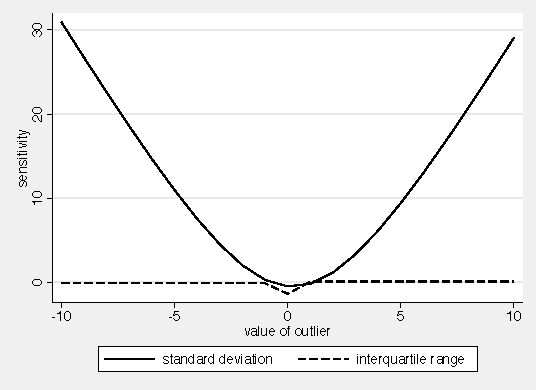
\epsfig{file=eps/2/5}
    \caption{Standardized sensitivity curves of the standard deviation and the interquartile range for a sample of $n=20$ random $\mathcal{N}(0,1)$ numbers}
    \label{fig:theory:SCscale}
\end{figure}

\index{subject}{sensitivity curve|)}

\subsubsection{The influence function}
\index{subject}{influence function|(textbf}

An intuitive way to introduce the \emph{influence function} (\stsc{IF}) of
functional $T$ at some distribution $F$ is to think of the influence function
as an asymptotic version of the \Index{sensitivity curve} of statistic $T_n=T(F_n)$
when the sample size $n$ grows, so that the empirical distribution function
$F_n$ tends to the underlying population distribution function $F$ (cf.\
\citealp{hampel:1974}). More precisely, the influence function is defined as
%
\begin{align*}
    \stsc{IF}(x; T, F) 
        &= \lim_{n\rightarrow\infty} \frac{T\left(\left(1-\frac{1}{n+1}\right) F + 
            \frac{1}{n+1} \Delta_x\right) - T(F)}{\frac{1}{n+1}} \\
        &= \lim_{\varepsilon\rightarrow 0} \frac{T\left((1-\varepsilon) F + 
            \varepsilon\Delta_x\right) - T(F)}{\varepsilon}
\end{align*}
%
where $\Delta_x$ is a probability distribution with all its mass at point
$x$. That is, the influence function measures the effect on $T$ of a
perturbation of $F$ obtained by adding a small probability mass at point $x$.
$\stsc{IF}(x;T,F)$ can be found for most functionals $T$. In
chapter~\ref{chap:stats} we will provide the influence functions
of various measures of location, scale, skewness and tails heaviness.

\index{subject}{influence function|)}

\subsubsection{The gross-error sensitivity}
\index{subject}{gross-error sensitivity|(textbf}

Since $\stsc{IF}(x; T, F)$ quantifies the influence on $T$ of an infinitesimal
contamination of the distribution $F$ at point $x$, it is a \emph{local}
measure of robustness. It may be completed by a more global measure, the
\emph{gross-error sensitivity} of $T$ at distribution $F$, defined as
\[
    \gamma^*(T, F) = \sup_x \left| \stsc{IF}(x; T, F) \right|
\]
$\gamma^*(T, F)$ evaluates to the biggest influence an outlier can have on
the functional $T$. With respect to robustness it is desirable to use an
estimator that is associated with a functional $T$ for which $\gamma^*(T, F)$ 
is finite (that is, for which the influence function is bounded).

\index{subject}{gross-error sensitivity|)}

\subsubsection{The local-shift sensitivity}
\index{subject}{local-shift sensitivity|(textbf}

The local-shift sensitivity is another tool related to the influence function;
it aims at measuring the effect of “wiggling” an observation, that is, of a
small perturbation as opposed to gross error. This is useful to asses the
effects of rounding, grouping, or other local inaccuracies.

Jumps in the \Index{influence function} (\stsc{IF}) indicate that a small
fluctuation of the value of $x$ can cause an abrupt change in the estimate.
Hence, from the perspective of robustness, we prefer a continuous \stsc{IF}
with an appropriately bounded derivative (wherever the derivative exists). 
To appreciate this kind of characteristic
of the \textit{IF}, we may determine the \emph{local-shift sensitivity}:
\[
    \lambda^*(T, F) = \sup_{x\neq y} \frac{|\stsc{IF}(y; T, F) - \stsc{IF}(x; T, F)|}
                                          {|y - x|}
\]

\index{subject}{local-shift sensitivity|)}

\subsubsection{The asymptotic variance of an estimator}
\index{subject}{asymptotic variance|(textbf}

The \Index{influence function} may also be used as a heuristic tool to determine the
asymptotic variance of the estimators. Indeed, under some regularity conditions
for the functional $T$, we have, under $F$,                                     \todo{Why is “under $F$” needed? 
                                                                                Isn't this obvious? And: What does “$\longrightarrow^d$” mean?
                                                                                “approximately distributed as”? or “asymptotically 
                                                                                distributed as”? or simply “distributed as”?
                                                                                Why not “$\sim$” or “$\stackrel{a}{\sim}$”?
                                                                                Furthermore: Why not include “$/n$” in the definition
                                                                                of \stsc{ASV}?}
\[
    \sqrt{n}\left(T(F_n) - T(F)\right) \longrightarrow^d \mathcal{N}\left(0, \stsc{ASV}(T, F)\right)
\]
where
\begin{equation}\label{eq:ASV}
    \stsc{ASV}(T, F) = \int_{-\infty}^\infty \stsc{IF}(x; T, F)^2 \dif F(x)
\end{equation}
(cf.\ \citealp[p. 85 and 226]{hampel:etal:1986}). Consequently, under $F$, the
interval
\[
    \left[ T(F_n) - z_{(1-\alpha/2)} \frac{\sqrt{\stsc{ASV}(T, F)}}{\sqrt{n}},\, 
           T(F_n) + z_{(1-\alpha/2)} \frac{\sqrt{\stsc{ASV}(T, F)}}{\sqrt{n}}\right]
\]
provides an asymptotic confidence interval for the parameter $T(F)$, at a
confidence level of $(1-\alpha)$\%. If the distribution $F$, and hence the
asymptotic variance $\stsc{ASV}(T, F)$, are not known, it is still possible to
obtain a confidence interval for $T(F)$ by an appropriate \Index{resampling} method.
                                                                                \todo{Hm, isn't it possible to simply use
                                                                                \stsc{IF} evaluated at the sample
                                                                                to get an estimate of \stsc{ASV}?
                                                                                (i.e. without resampling) That is, 
                                                                                evaluate \stsc{IF} at each observed
                                                                                $x$ using $F_n$ instead of $F$ and 
                                                                                then compute the variance from these
                                                                                values. At least this is an approach 
                                                                                I saw in other research.}

\index{subject}{asymptotic variance|)}

\subsection{The breakdown point}
\index{subject}{breakdown point|(textbf}
\label{subsec:theory:BP}

The \Index{sensitivity curve} shows how an estimator reacts to the introduction
of one single outlier. Some estimators cannot resist even against a
single outlier. As we have seen, this is the case for the mean and the
\Index{standard deviation}. Other estimators, such as the \Index{median} and
the \Index{interquartile range}, are robust against this type of
contamination because their \Index{sensitivity curve} (\stsc{SC}) is
bounded. Possibly, however, the number of outliers in a sample is so large that
even estimators with a bounded \stsc{SC} can no longer resist their effect.
Hence, to evaluate different estimators, it is important to know what the
amount of contamination is an estimator can tolerate. The
\emph{breakdown point} is a measure for such \emph{resistance} of an estimator.
It quantifies, roughly, the smallest amount of contamination in the
sample that may cause the estimator to take on arbitrary values. Its definition
is as follows.

\subsubsection{The finite-sample breakdown point}
\index{subject}{breakdown point!finite-sample|(textbf}

The breakdown point $\epsilon_n^*(T_n; \mathbf{X}_n)$ of the statistic
$T_n = T_n(x_1, \dots, x_n) = T(F_n)$ at the sample $\mathbf{X}_n 
= \{x_1, \dots, x_n\}$ refers to the smallest proportion of observations
in $\mathbf{X}_n$ that need to be replaced to cause the value of the
statistic to be arbitrarily large or small, and hence, to make the statistic
worthless or meaningless. Note that, typically, $\epsilon_n^*$ is
independent of $x_1, \dots, x_n$.

More formally, for a univariate location estimator $T_n$, which breaks down
if its value becomes arbitrarily large, we may define the (finite-sample)
breakdown point as follows (see \citealp{hampel:stahel:1982};
\citealp{donoho:huber:1983}). In a given sample $\mathbf{X}_n = \{x_1,
\dots, x_n\}$, let us replace $m$ data points $x_{i_1}, \dots, x_{i_{m}}$
by arbitrary values $y_1, \dots, y_{m}$; let us call the new data set        \todo{I assume $\min\{x; y\}$ means “find the smallest $x$ for which $y$ is true”. This should be explained somewhere.}%
$\mathbf{Z}_n = \{z_1, \dots, z_n\}$. Then the \emph{(finite-sample
gross-error) breakdown point} of the estimator is%
\[
    \epsilon_n^{\ast}(T_n; \mathbf{X}_n) 
    = \min \left\{\frac{m}{n}; \max_{i_i, \dots, i_{m}} \sup_{y_1, \dots, y_{m}} 
      \left|T_n(z_1, \dots, z_n)\right| =\infty \right\}
\]

Following the same idea, we will say that a scale estimator breaks down if it
takes on a value that is arbitrarily large (scale explosion) or close to zero
(scale implosion). Furthermore, a \Index{skewness} or \Index{kurtosis}
estimator, which is bounded by $[-1, 1]$, breaks down if the absolute value of
the estimate attains the value of 1.

\begin{stexample}
If the $i$th observation among $x_1, \dots, x_n$ goes to infinity, the \Index{mean}
$\mu$ and the \Index{standard deviation} $\sigma$ go to infinity as well. This
means that the finite-sample breakdown point of these two statistics is $1/n$.
In contrast, the finite-sample breakdown point of the \Index{median} $Q_{0.5}$ is
$\frac{(n/2)}{n}$ if $n$ is even and $\frac{(n+1)/2}{n}$ if $n$ is odd. That is,
half the data or a bit more must be replaced to make the \Index{median} take on arbitrary
values. The finite-sample breakdown point of the \Index{interquartile range}
$\stsc{IQR}$ is equal to $\frac{\lfloor n/4 \rfloor + 1}{n}$, where
$\lfloor n/4 \rfloor $ denotes the integer part of $n/4$. That is, a bit more than 
one fourth of the data needs to be replaced to make the \stsc{IQR} break down.
\end{stexample}

\index{subject}{breakdown point!finite-sample|)}


\subsubsection{The asymptotic breakdown point}
\index{subject}{breakdown point!asymptotic|(textbf}

The \emph{asymptotic breakdown point} $\epsilon^*(T, F)$ of the functional
$T$ under the distribution $F$ is defined as
\[
    \epsilon^*(T, F) = \lim_{n\rightarrow\infty} \epsilon_n^*(T_n; \mathbf{X}_n)
\]
with the $x_i$'s sampled from $F$ (cf.\ \citealp{hampel:1971}).               \todo{Maybe give more details: max $\epsilon$ in 
                                                                                $(1-\epsilon)F+\epsilon G$ with any $G$ before $T$ 
                                                                                breaks down.}

\index{subject}{breakdown point!asymptotic|)}
\index{subject}{breakdown point|)}

\subsection{Gaussian efficiency}
\index{subject}{Gaussian efficiency|(textbf}

In general, if $F$ it is known, the ML-estimator for that $F$ is most efficient
(see above). Furthermore, for $F$ equal Gaussian, the mean is the ML-estimator
and hence most efficient. Robust estimators should not only be efficient with
respect to Gaussian, but for a wide variety of distributions. However, Gaussian
efficiency is also important if robust estimators are viewed as competitors of
standard estimators. Hence it is often good to know (relative) Gaussian
efficiency and then complement this with relative efficiencies for other
distributions.

\alert{[Give formal definitions etc. This is not only about Gaussian
efficiency. For example, the mean has high variance under fat-tails
distributions; robust estimators can have better efficiency in such cases...]}

\index{subject}{Gaussian efficiency|)}

\subsection{Aspects of Interpretation}

\alert{[What about asymmetric distributions and interpretation? (e.g.
Median vs. Mean) Need to address such aspects. The point is that robust
estimators often estimate something that is conceptually different than the
nonrobust counterpart (or something where robust and nonrobust counterparts
coincide only in special situations, such as in a symmetric distribution or in
a normal distribution).]}

\subsection{Summary}

How do we choose a good (robust) estimator? We are clearly interested in estimators with

\begin{enumerate}
    \item a \emph{bounded} (low \Index{gross-error sensitivity})
    and \emph{smooth} (low \Index{local-shift sensitivity}) \emph{\Index{influence function}} 

    \item and a \emph{high \Index{breakdown point}}.
\end{enumerate}

\index{subject}{Fisher consistency|(textbf}
Moreover, we are generally considering estimators that are
\emph{(Fisher-)consistent}. To specify this property, let us consider a
\emph{parametric model}, that is, let us assume that the underlying
population distribution $F$ has a specified form but depends on one or more
unknown parameters. Formally: $F \in \{F_{\theta}; \theta\in\Theta\}$. For
instance, in the location model, the underlying distribution is assumed to be
$F_\mu(x) = F_0(x - \mu)$, where $F_0$ is a generic
distribution function. In the location-scale model, the population
distribution is $F_{\mathbf{\theta}}(x) = F_0\left(\frac{x-\mu}{\sigma}\right)$ 
with $\mathbf{\theta} = (\mu, \sigma)'$. In this parametric
context, an estimator $T_n = T(F_n)$ of the parameter $\theta$ of a
parametric family is said to be \emph{Fisher-consistent} if this estimator
is associated with a functional $T$ such that, for $n \rightarrow \infty$,      \todo{I don't really understand. Is Fisher-consistency
                                                                                defined with respect to a specified $F_0$, 
                                                                                or does it mean that the 
                                                                                relation holds in general, for any arbitrary $F_0$?}
\[
    T_n = T(F_n) \longrightarrow^\text{P} T(F_{\theta}) = \theta 
    \qquad
    \text{for all $\theta\in\Theta$}
\]
where $\longrightarrow^\text{P}$ denotes the convergence in probability.
That is, irrespective of the value of $\theta$, a \emph{Fisher-consistent} 
estimator will always converge to $\theta$.
\index{subject}{Fisher consistency|)}

Finally, we are also looking for estimators that are as \emph{efficient}
as possible at an assumed model. In general, compromises between robustness and 
efficiency must be made to achieve good overall performance, as is shown in 
the following section.



\endinput
